% !TEX TS-program = pdflatex
% !TEX encoding = UTF-8 Unicode

% This is a simple template for a LaTeX document using the "article" class.
% See "book", "report", "letter" for other types of document.

\documentclass[11pt]{article} % use larger type; default would be 10pt

\usepackage[utf8]{inputenc} % set input encoding (not needed with XeLaTeX)

%%% Examples of Article customizations
% These packages are optional, depending whether you want the features they provide.
% See the LaTeX Companion or other references for full information.

%%% PAGE DIMENSIONS
\usepackage{geometry} % to change the page dimensions
\geometry{a4paper} % or letterpaper (US) or a5paper or....
% \geometry{margin=2in} % for example, change the margins to 2 inches all round
% \geometry{landscape} % set up the page for landscape
%   read geometry.pdf for detailed page layout information

\usepackage{graphicx} % support the \includegraphics command and options

% \usepackage[parfill]{parskip} % Activate to begin paragraphs with an empty line rather than an indent

%%% PACKAGES
\usepackage{booktabs} % for much better looking tables
\usepackage{array} % for better arrays (eg matrices) in maths
\usepackage{paralist} % very flexible & customisable lists (eg. enumerate/itemize, etc.)
\usepackage{verbatim} % adds environment for commenting out blocks of text & for better verbatim
\usepackage{subfig} % make it possible to include more than one captioned figure/table in a single float
% These packages are all incorporated in the memoir class to one degree or another...

\usepackage[polish]{babel}	
\usepackage{polski}
\usepackage[T1]{fontenc}
\frenchspacing	

\usepackage{indentfirst}


%%% HEADERS & FOOTERS
\usepackage{fancyhdr} % This should be set AFTER setting up the page geometry
\pagestyle{fancy} % options: empty , plain , fancy
\renewcommand{\headrulewidth}{0pt} % customise the layout...
\lhead{}\chead{}\rhead{}
\lfoot{}\cfoot{\thepage}\rfoot{}

%%% SECTION TITLE APPEARANCE
\usepackage{sectsty}
\allsectionsfont{\sffamily\mdseries\upshape} % (See the fntguide.pdf for font help)
% (This matches ConTeXt defaults)

%%% ToC (table of contents) APPEARANCE
\usepackage[nottoc,notlof,notlot]{tocbibind} % Put the bibliography in the ToC
\usepackage[titles,subfigure]{tocloft} % Alter the style of the Table of Contents
\renewcommand{\cftsecfont}{\rmfamily\mdseries\upshape}
\renewcommand{\cftsecpagefont}{\rmfamily\mdseries\upshape} % No bold!

%%% END Article customizations

%%% The "real" document content comes below...

\title{Sztuczne Sieci Neuronowe \\ \large Sprawozdanie z projektu}
\author{Łukasz Rados, Wojciech Kusa \\ Wydział Fizyki i Informatyki Stosowanej \\ Akademia Górniczo-Hutnicza im. Stanisława Staszica w Krakowie}
%\date{} % Activate to display a given date or no date (if empty),
         % otherwise the current date is printed 

\begin{document}
\maketitle

\section{Wprowadzenie}

Celem opisywanego projektu było zaimplementowanie i próba nauczenia sieci neuronowych grania w prostą grę komputerową. 

Genezą projektu jest publikacja [1], w której autorzy próbują nauczyć sieć neuronową za pomocą metody tzw. deep learning algorytmów grania w różne gry komputerowe wydane na platformę Atari. Naszą motywacją było stworzenie gry komputerowej wzorującej się na grze \textit{TRex Runner}, która znajduje się w przeglądarce Google Chrome, a następnie zaimplementowanie takiej struktury sieci neuronowej, która byłaby w stanie nauczyć się skutecznie grać w tę grę. 

Przetestowane zostały różne rodzaje sieci?? oraz wpływ technik uczenia na jej jakość działania??.

Projekt został wykonany w języku Python z wykorzystaniem bibliotek do obliczeń numerycznych NumPy, SciPy oraz biblioteki wspomagającej proces tworzenia gier PyGame.


\section{Podstawy teoretyczne}



\section{Gra}


Zaimplementowana została gra komputerowa "Dinosaur".

\begin{figure}[h]
\centering
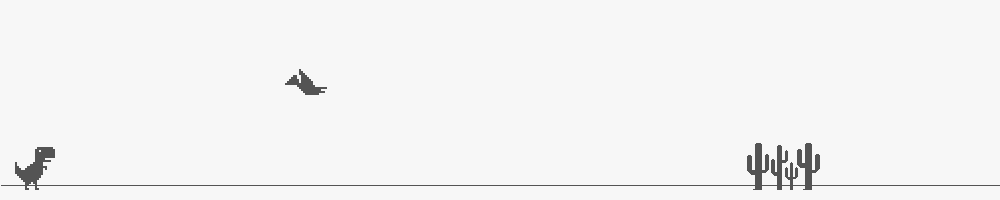
\includegraphics[width=10cm]{images/dinosaur_1}
\caption{Stan planszy, w którym nie ma działania pozwalającego na przeżycie dinozaura.} \label{fig:dinosaur_1}
\end{figure}

\begin{figure}[h]
\centering
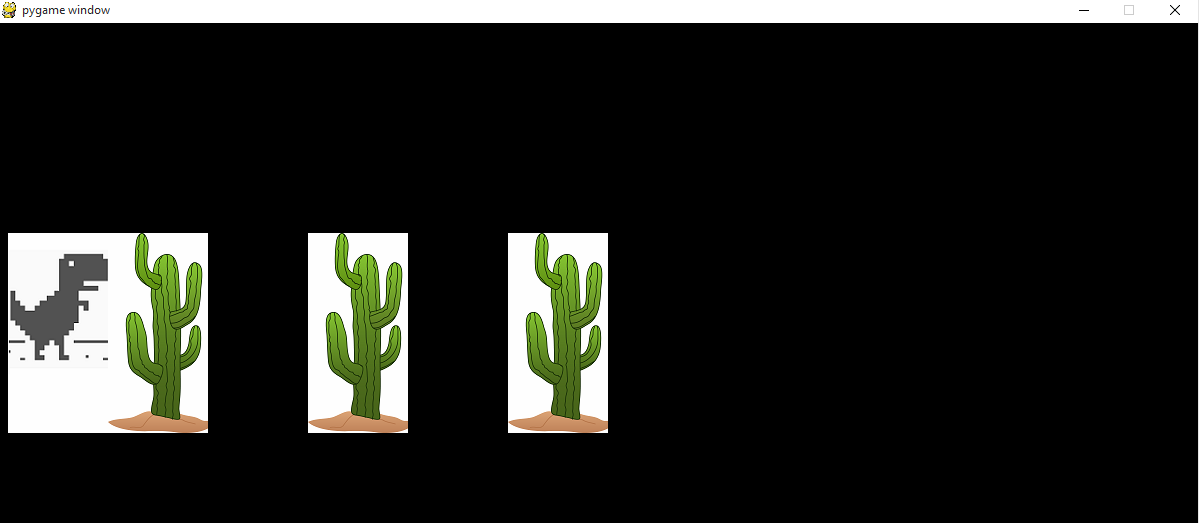
\includegraphics[width=10cm]{images/dinosaur_2}
\caption{Stan planszy, w którym nie ma działania pozwalającego na przeżycie dinozaura.} \label{fig:dinosaur_2}
\end{figure}

\begin{figure}[h]
\centering
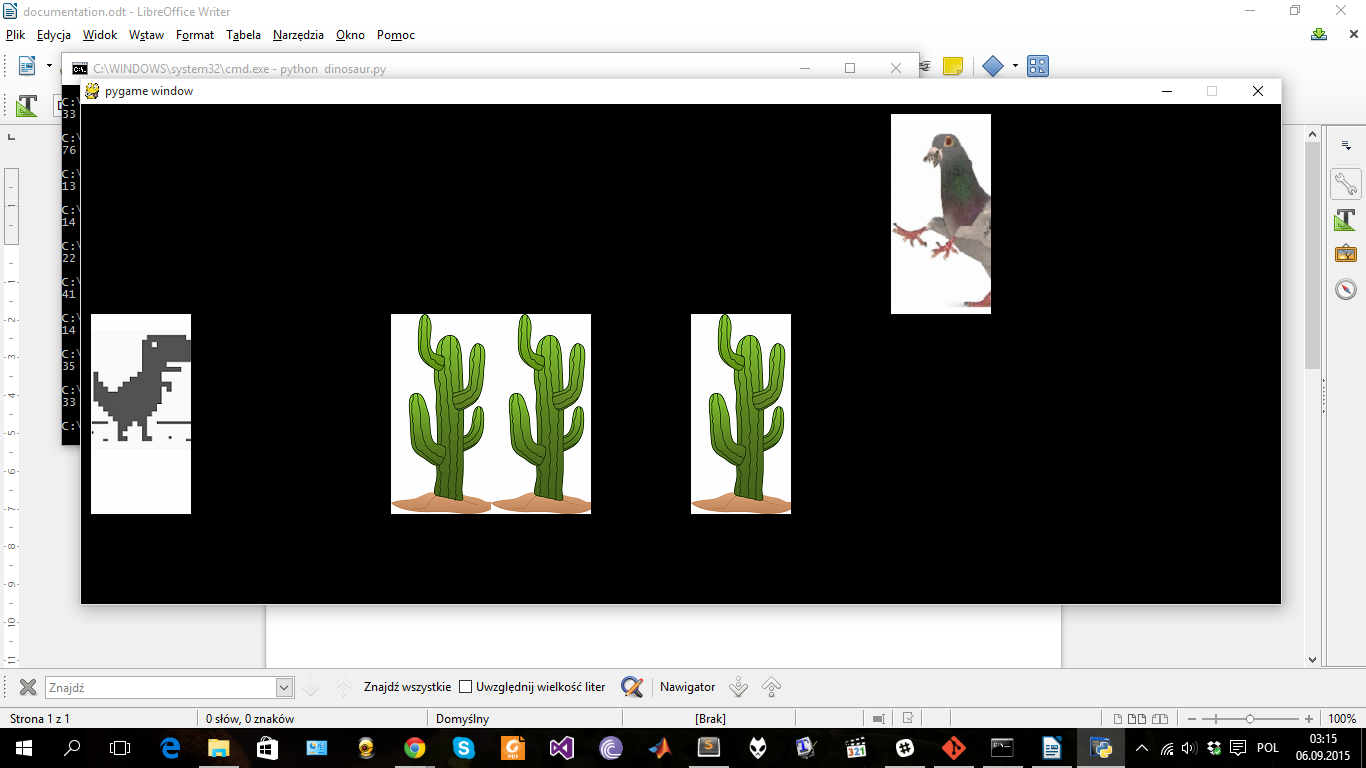
\includegraphics[width=10cm]{images/dinosaur_3}
\caption{Wymagany bardzo dobry refleks (dla komputera to nie jest przeszkoda).} \label{fig:dinosaur_3}
\end{figure}

\section{Bibliografia}

\begin{enumerate}
\item V Mnih, K Kavukcuoglu, D Silver, A Graves, I Antonoglou, D Wierstra, M Riedmiller - Playing Atari with Deep Reinforcement Learning.  NIPS 2013 Deep Learning Workshop

\end{enumerate}

\end{document}
